\section{AVR Timers}

%----------------------------------------------------------------------------------------
%	DEFINITION SUBESCTION
%----------------------------------------------------------------------------------------
\subsection{Definition}
Timers are standard features of almost every microcontroller. So it is very important to learn their use. Since an AVR microcontroller has very powerful and multifunctional timers, the topic of timer is somewhat “vast”. Moreover there are many different timers on chip. So this section on timers will be multipart. I will be giving basic introduction first.

%----------------------------------------------------------------------------------------
%	WHAT IS TIMER SUBESCTION
%----------------------------------------------------------------------------------------

\subsection{What is a timer ?}
A timer in simplest term is a register. Timers generally have a resolution of 8 or 16 Bits. So a 8 bit timer is 8Bits wide so capable of holding value withing 0-255. But this register has a magical property ! Its value increases/decreases automatically at a predefined rate (supplied by user). This is the timer clock. And this operation does not need CPU’s intervention.
\\\\
\centerline{
	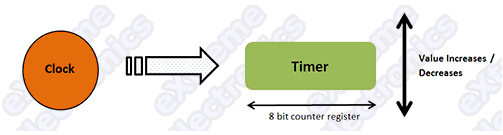
\includegraphics[width=0.6\textwidth]{overview/images/timer1.png}
}

%----------------------------------------------------------------------------------------
%	BASIC TIMER OPERATION SUBESCTION
%----------------------------------------------------------------------------------------

\subsection{Basic operation of a timer}
Since Timer works independently of CPU it can be used to measure time accurately. Timer upon certain conditions take some action automatically or inform CPU. One of the basic condition is the situation when timer OVERFLOWS i.e. its counted upto its maximum value (255 for 8 BIT timers) and rolled back to 0. In this situation timer can issue an interrupt and you must write an Interrupt Service Routine (ISR) to handle the event.
\\\\
\centerline{
	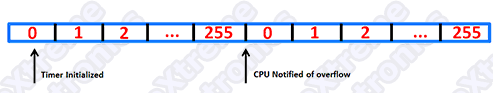
\includegraphics[width=0.6\textwidth]{overview/images/timer2.png}
}

%----------------------------------------------------------------------------------------
%	USING 8 BIT TIMER SUBESCTION
%----------------------------------------------------------------------------------------

\subsection{Using the 8 bit timer (TIMER0)}
The ATmega16 and ATmega32 has three different timers of which the simplest is TIMER0. Its resolution is 8 BIT i.e. it can count from 0 to 255. Note: Please read the “Internal Peripherals of AVRs” to have the basic knowledge of techniques used for using the OnChip peripherals(Like timer !) The Prescaler The Prescaler is a mechanism for generating clock for timer by the CPU clock. As you know that CPU has a clock source such as a external crystal of internal oscillator. Normally these have the frequency like 1 MHz,8 MHz, 12 MHz or 16MHz(MAX). The Prescaler is used to divide this clock frequency and produce a clock for TIMER. The Prescaler can be used to get the following clock for timer. No Clock (Timer Stop). No Prescaling (Clock = FCPU) FCPU/8 FCPU/64 FCPU/256 FCPU/1024 Timer can also be externally clocked but I am leaving it for now for simplicity.

%----------------------------------------------------------------------------------------
%	TIMER0 REGISTERS SUBESCTION
%----------------------------------------------------------------------------------------

\subsection{TIMER0 registers}
As you may be knowing from the article “Internal Peripherals of AVRs” every peripheral is connected with CPU from a set of registers used to communicate with it. The registers of TIMERs are given below.

TCCR0 – Timer Counter Control Register. This will be used to configure the timer.
\\\\
\centerline{
	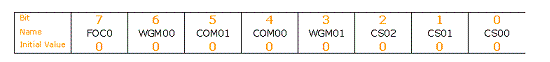
\includegraphics[width=0.6\textwidth]{overview/images/timer3.png}
}

%----------------------------------------------------------------------------------------
%	TIMER COUNTER CONTROLL SUBESCTION
%----------------------------------------------------------------------------------------
\newpage
\subsection{Timer counter control register TCCR0}
As you can see there are 8 Bits in this register each used for certain purpose. For this tutorial I will only focus on the last three bits CS02 CS01 CS00 They are the CLOCK SELECT bits. They are used to set up the Prescaler for timer.
\\\\
\centerline{
	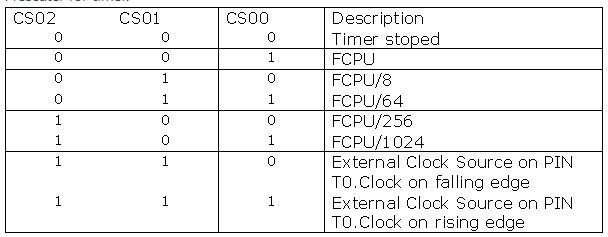
\includegraphics[width=0.6\textwidth]{overview/images/timer4.png}
}

%----------------------------------------------------------------------------------------
%	TCNT0 SUBESCTION
%----------------------------------------------------------------------------------------
\subsection{TCNT0 – Timer counter 0}
\centerline{
	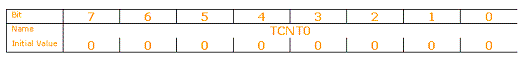
\includegraphics[width=0.6\textwidth]{overview/images/timer5.png}
}

%----------------------------------------------------------------------------------------
%	TIMER INTERRUPT MASK SUBESCTION
%----------------------------------------------------------------------------------------
\subsection{Timer interrupt mask register (TIMSK)}
\centerline{
	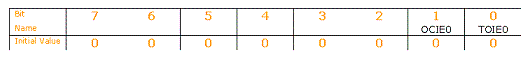
\includegraphics[width=0.6\textwidth]{overview/images/timer6.png}
}

This register is used to activate/deactivate interrupts related with timers. This register controls the interrupts of all the three timers. The last two bits (BIT 1 and BIT 0) Controls the interrupts of TIMER0. TIMER0 has two interrupts but in this article I will tell you only about one(second one for next tutorial). TOIE0 : This bit when set to “1” enables the OVERFLOW interrupt. Now time for some practical codes !!! We will set up timer to at a Prescaler of 1024 and our FCPU is 16MHz. We will increment a variable “count” at every interrupt(OVERFLOW) if count reaches 61 we will toggle PORTC0 which is connected to LED and reset “count= 0”. Clock input of TIMER0 = 16MHz/1024 = 15625 Hz Frequency of Overflow = 15625 /256 = 61.0352 Hz if we increment a variable “count” every Overflow when “count reach 61” approx one second has elapse.

